The shadow suppression is performed in a fashion similar to what is mentioned in the paper by Woods \cite{Wood}. The suppression if performed using the Hue- Saturation- Value- (HSV) mapping, The HSV mapping was chosen since it gives very small amounts of false positives and a manageable number of false negatives, while at the same time being fairly simple. We make the assumption that a if a pixel is shadowed the hue remains constant, while there is a decrease in both the value and saturation channels compared to the most likely background at the time.


\subsubsection{Implementation}
The Shadow Suppression function is called with a reference to \emph{frame} object containing both a processed version of the probability map, the current frame image as well as the most likely background. The first step is to remap the current frame image and the background model to the HSV-space. The suppression is performed by comparing all H- S- and V-values in the remapped images. If a pixel marked as foreground by the background model has a the same hue but lower saturation and value in the image than in the background model, it is assumed to be caused by a shadow, (eq. 3.19 in Wood \cite{Wood}). All probability map pixels assumed to be shadows are set to zero, and the shadow suppression is thereby finished.

\subsubsection{Parameters}
The parameters that need to be specified in the shadow suppression are the threshold values for the different channels, $\tau_H$, $\tau_S$, $\alpha$ and $\beta$. Let i denote the current image and m the current background model. In order for a pixel to be classified as shadow, all of the following three constraints have to be fulfilled:

\begin{equation}
	|H_i - H_m| < \tau_H
	\label{eq:H}
\end{equation}
\begin{equation}
	S_i - S_m < \tau_S
	\label{eq:S}
\end{equation}
\begin{equation}
	\alpha_V < \frac{V_i}{V_m} < \beta_V
	\label{eq:V}
\end{equation}

The paramter setting depend on the scene that is being observed. For example in figure \ref{fig:shadow_suppression_fig} where most of the shadows are cast on a gray road (hue $\approx 0$), a rather large $\tau_H$ is required. Also, since the shadows are not so profound, alpha can be raised, causing lower false positives for dark objects. (a problem occuring, for example, in the Renova 0000 sequence).

\newpage
\begin{figure}[htb]
	\centering
	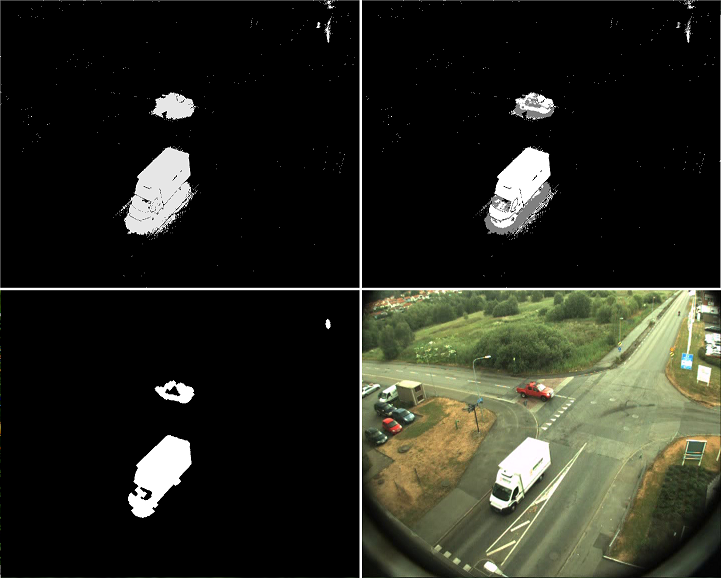
\includegraphics[width=\linewidth]{images/ShadowRenova0002.png}
	\caption{\textit{Renova image sequence 0002, frame 217. 
	From the top and right: Background model output, Model output with marked shadow pixels (gray), final foreground image and actual video frame}}
	\label{fig:shadow_suppression_fig}  %Skapar referens till figuren
\end{figure}
